% --------------------------------------------------------------
% This is all preamble stuff that you don't have to worry about.
% Head down to where it says "Start here"
% --------------------------------------------------------------
 
\documentclass[12pt]{article}
 
\usepackage[margin=1in]{geometry} 
\usepackage{amsmath,amsthm,amssymb}
\usepackage{graphicx} 
\usepackage{float}
\usepackage{booktabs}
\usepackage{subcaption}
\usepackage{longtable}

\newcommand{\N}{\mathbb{N}}
\newcommand{\Z}{\mathbb{Z}}
 
\newenvironment{theorem}[2][Theorem]{\begin{trivlist}
\item[\hskip \labelsep {\bfseries #1}\hskip \labelsep {\bfseries #2.}]}{\end{trivlist}}
\newenvironment{lemma}[2][Lemma]{\begin{trivlist}
\item[\hskip \labelsep {\bfseries #1}\hskip \labelsep {\bfseries #2.}]}{\end{trivlist}}
\newenvironment{exercise}[2][Exercise]{\begin{trivlist}
\item[\hskip \labelsep {\bfseries #1}\hskip \labelsep {\bfseries #2.}]}{\end{trivlist}}
\newenvironment{problem}[2][Problem]{\begin{trivlist}
\item[\hskip \labelsep {\bfseries #1}\hskip \labelsep {\bfseries #2.}]}{\end{trivlist}}
\newenvironment{question}[2][Question]{\begin{trivlist}
\item[\hskip \labelsep {\bfseries #1}\hskip \labelsep {\bfseries #2.}]}{\end{trivlist}}
\newenvironment{corollary}[2][Corollary]{\begin{trivlist}
\item[\hskip \labelsep {\bfseries #1}\hskip \labelsep {\bfseries #2.}]}{\end{trivlist}}

\newenvironment{solution}{\begin{proof}[Solution]}{\end{proof}}
\setlength{\parindent}{0pt}
\begin{document}
 
% --------------------------------------------------------------
%                         Start here
% --------------------------------------------------------------
 
\title{Nano Bartender}
\author{Maragliano Gianluca, Perri Raffaele, Seipl Paul Leopold\\ %replace with your name
Edge Computing in the IoT}

\maketitle

\section{Introduction}

\section{Hardware Architecture \& Sensors}
The system relies on a sensor fusion approach to capture distinct physical and optical properties of liquids, as well as the motion of the device itself.
\subsection*{Microcontroller: Arduino Nano 33 BLE Sense}
The core processing unit is the Arduino Nano 33 BLE Sense. It was chosen for its small form factor and its rich set of onboard sensors, specifically the color sensor, which is crucial for this application. It handles sensor data acquisition, runs the Edge Impulse inference engine, and manages state transitions.
\subsection*{Capacitive Soil Moisture Sensor v1.0}
\begin{figure}[H]
    \centering
    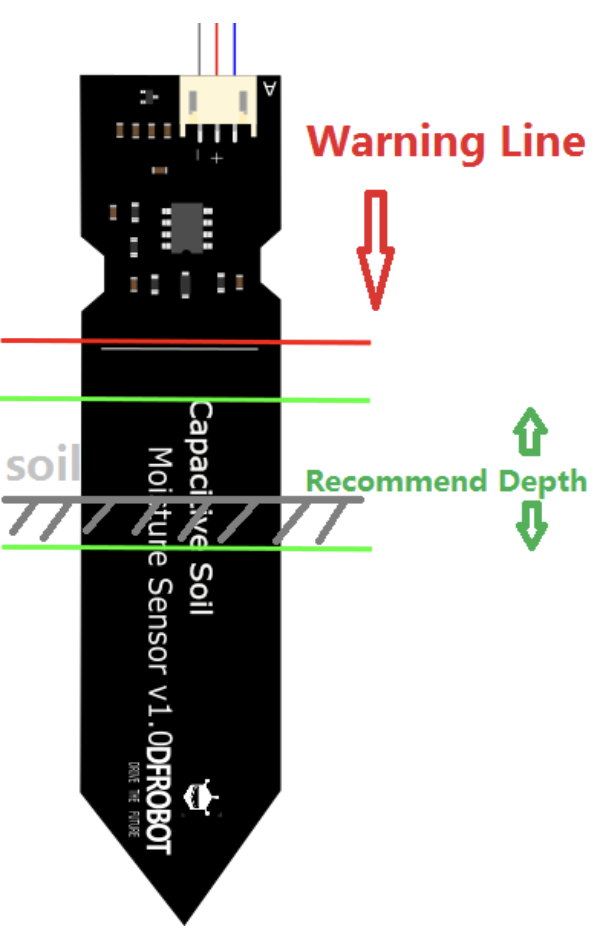
\includegraphics[width=0.2\textwidth]{images/capacitive.png}
    \caption{Capacitive Soil Moisture Sensor v1.0}
\end{figure}
\textbf{Specfications:}
\begin{itemize}
    \item Operating Voltage: $3.3 \sim 5.5$ VDC
    \item Output Voltage: $0 \sim 3.0$ VDC
    \item Operating Current: 5mA
    \item Interface: PH2.0-3P
    \item Dimensions: $3.86 \times 0.905$ inches (L x W)
    \item Weight: 15g
\end{itemize}
\textbf{Purpose:} To measure the dielectric permittivity of the liquid.\\
\textbf{Mechanism:} While typically used for soil, this sensor measures capacitance changes based on the medium it is submerged in. Different liquids have different dielectric constants, resulting in distinct analog voltage outputs.\\
\textbf{Characteristics:} Corrosion-resistant probe, analog output interface.
\subsection*{IMU (MPU-6886)}
\begin{figure}[H]
    \centering
    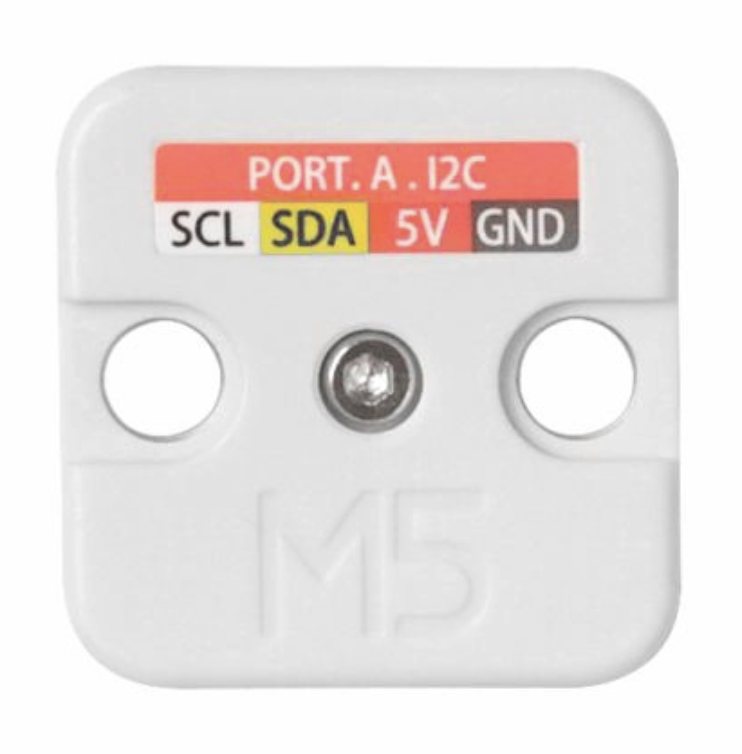
\includegraphics[width=0.2\textwidth]{images/IMU.png}
    \caption{MPU-6886 6-axis IMU}
\end{figure}
\textbf{Specifications:}
\begin{itemize}
    \item 3-axis gravity accelerometer and 3-axis gyroscope
    \item On-chip temperature sensor
    \item 1KB FIFO
    \item Supports low power consumption
    \item Development platforms: Arduino, UIFlow (Blockly, Python)
    \item 2 x LEGO-compatible holes
\end{itemize}
    \textbf{Purpose:} To detect motion and orientation for "Drinking Mode."\\
    \textbf{Mechanism:} The MPU-6886 is a 6-axis MotionTracking device that combines a 3-axis gyroscope and a 3-axis accelerometer.\\
    \textbf{Role in Project:} It detects the specific tilt angle and stability associated with the action of taking a sip.
\subsection*{Wired Push Button}
\begin{figure}[H]
    \centering
    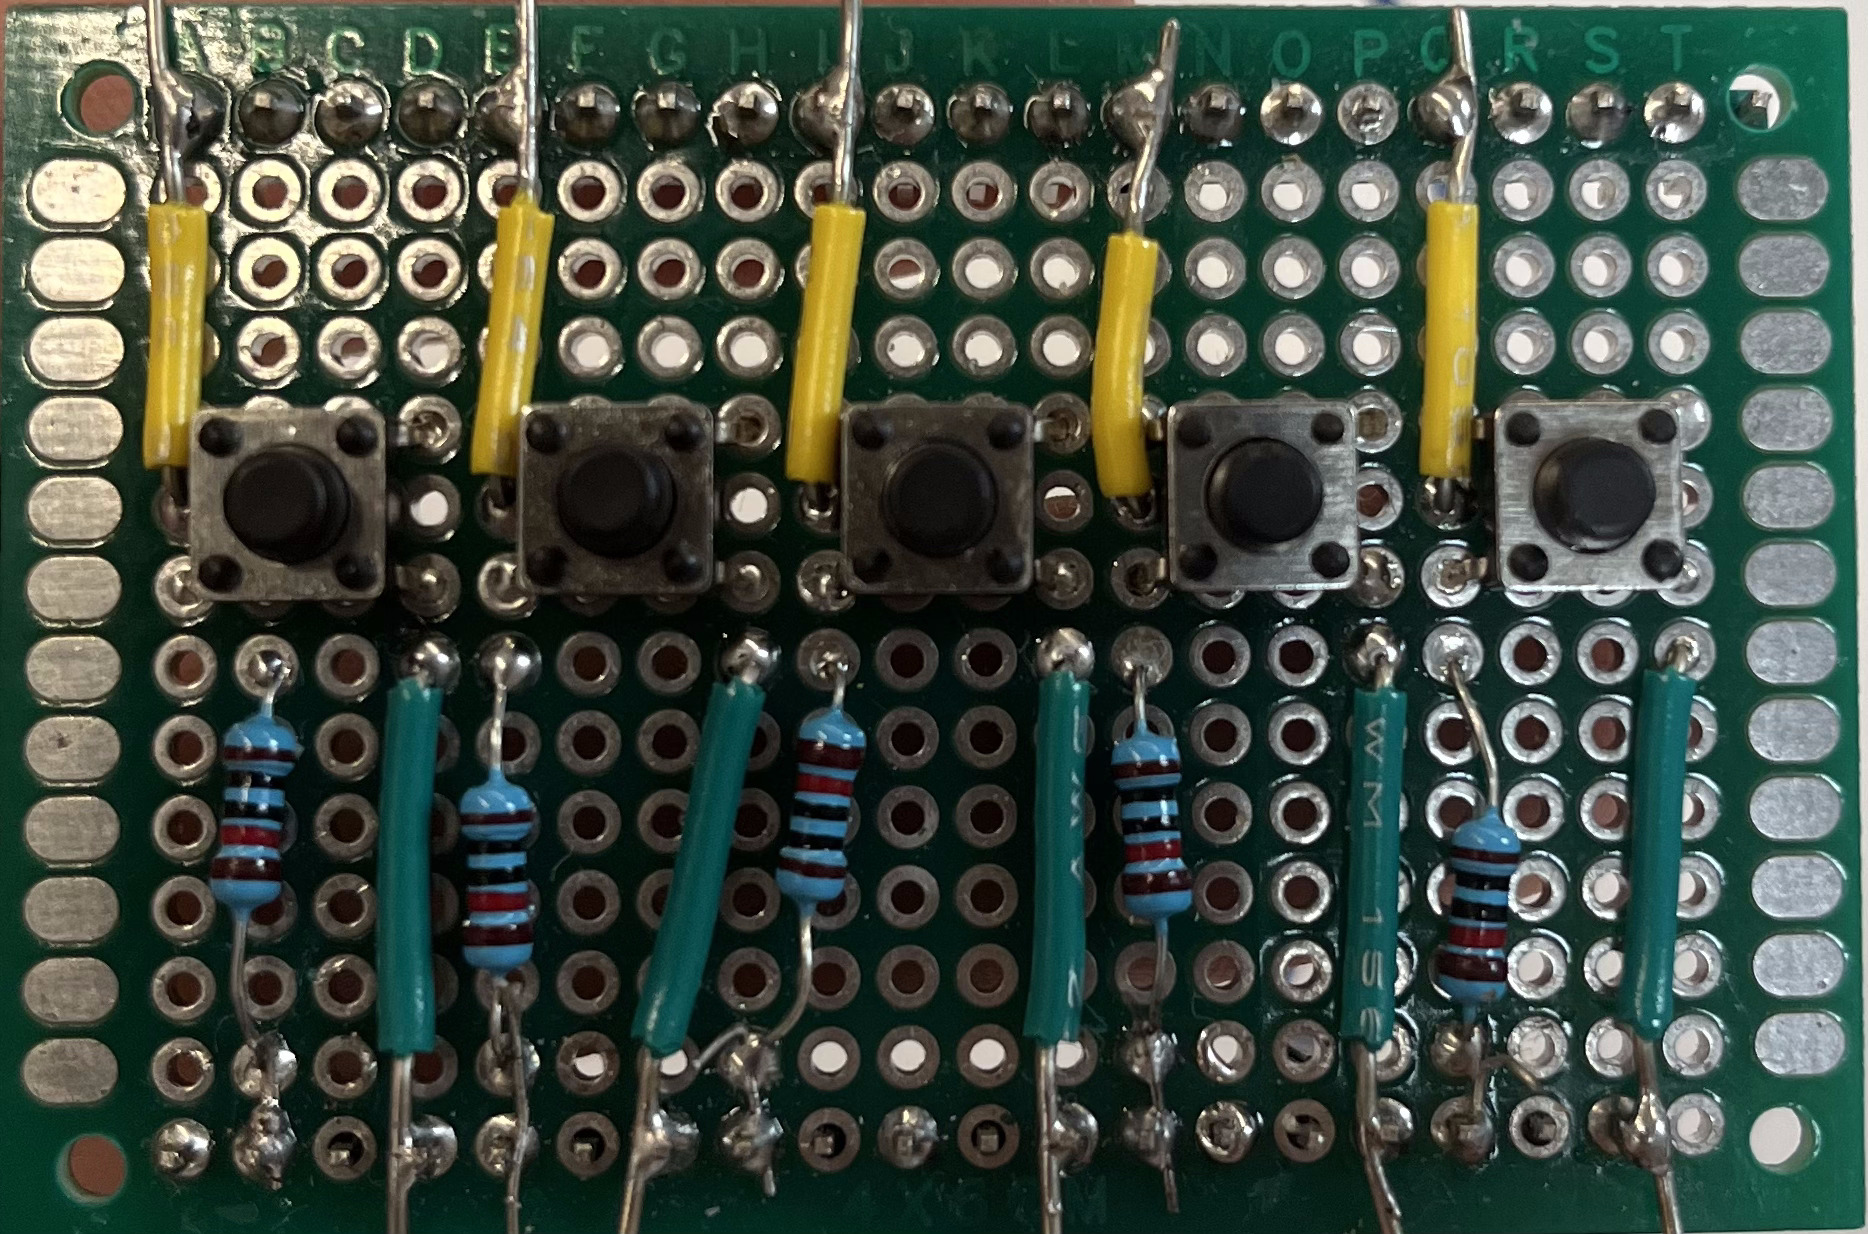
\includegraphics[width=0.3\textwidth]{images/button.jpg}
    \caption{Wired Push Button}
\end{figure}
\begin{itemize}
    \item Purpose: User input for state management.
    \item Function: Acts as a physical interrupt or toggle switch to transition the system between "Classification Mode" (identifying the drink) and "Drinking Mode" (monitoring consumption).
\end{itemize}

\section{System Design \& Integration}
The system logic is divided into two distinct operational modes triggered by user interaction.
\subsection{Data Acquisition Strategy}
To ensure reliable data for classification, raw sensor values were not used directly. Instead, a moving average filter was implemented:
\begin{itemize}
    \item Sampling: The system collects 5 consecutive readings from both the Capacitive Sensor and the RGB Color Sensor.
    \item Averaging: These values are averaged to reduce signal noise and outliers, providing a stable feature vector for the classifier.
\end{itemize}
\subsection{Operational Flow}
\begin{enumerate}
    \item Idle/Start: System initializes sensors and connects to the web interface.
    \item Classification Mode: The device reads capacitance and RGB values. The on-device TinyML model infers the liquid type.
    \item Mode Switch: Pressing the wired button toggles the state.
    \item Drinking Mode: The system continuously monitors the MPU-6886. If the pitch/roll exceeds a defined threshold (indicating a tilt), a timer starts. The timer stops when the device returns to a flat position, calculating the total "sip duration."
\end{enumerate}

\section{Machine Learning Implementation}
The core intelligence of the Drink Analyzer is a classifier trained using Edge Impulse.

Dataset Creation:
\begin{itemize}
    \item Classes: Water, Beer, Wine, Aperol, Rum.
    \item Features: Capacitance (Analog Value), Red, Green, Blue (Color Channels).
    \item Data Collection: A rigorous data collection phase was conducted, capturing varied samples for each liquid to ensure robustness.
    \item Model Architecture: A Neural Network classifier was designed to take the 4 input features and output a probability distribution across the 5 classes.
    \item Performance: The model achieved 100\% accuracy on the training set, indicating distinct separability between the chosen liquids based on color and capacitance.
    \item Deployment: The trained model was exported as an Arduino library and deployed directly to the Nano 33 BLE Sense, allowing for offline, low-latency inference.
\end{itemize}

\section{User Interface (Web Application)}
To enhance usability, a Python-based web application was developed.\\
Connectivity: The Arduino sends classification results and sip duration data via Bluetooth to the host computer.\\
Dashboard: The Python app visualizes:
\begin{itemize}
    \item Current Drink Detected.
    \item Session Stats (Duration of current sip).
\end{itemize}

\section{Design Choices}
This section outlines the critical architectural and methodological decisions made during the development of the Drink Analyzer. These choices were driven by hardware constraints, sensor capabilities, and the practical requirements of training a robust machine learning model.
\subsection{Sensor Selection and Exclusion: The DS18B20}
Initially, the hardware design included a DS18B20 digital temperature sensor (Figure~\ref{fig:DS18B20}). The hypothesis was that the temperature of the liquid might significantly alter its dielectric properties, thereby affecting the readings from the Capacitive Soil Moisture Sensor.
\begin{figure}[H]
    \centering
    \includegraphics[width=0.5\textwidth]{images/ds18b20.png}
    \caption{DS18B20 Digital Temperature Sensor}
    \label{fig:DS18B20}
\end{figure}
However, during the preliminary testing phase, we decided to exclude this sensor for two main reasons:
\begin{enumerate}
    \item Incompatibility: We encountered significant library and protocol incompatibilities between the standard OneWire libraries used for the DS18B20 and the architecture of the Arduino Nano 33 BLE Sense (built on the nRF52840 microcontroller). This created conflicts that hindered the stability of the system.
    \item Lack of Correlation: Empirical testing revealed that for the temperature ranges typical of drinking beverages (approx. 4°C to 25°C), the variation in temperature did not produce a statistically significant change in the capacitive values captured by our specific sensor. The added complexity of debugging the compatibility issues outweighed the negligible value added to the feature set.
\end{enumerate}

\subsection{Feature Engineering: RGB Ratios vs. Raw Values}

A crucial design choice was made regarding the processing of color data. The APDS-9960 sensor on the Nano 33 BLE Sense provides raw counts for Red, Green, Blue, and Clear light.

Instead of feeding these raw integers directly into the neural network, we opted to calculate the ratio of each color channel relative to the total light intensity.

\textbf{Reasoning:} Raw values are highly susceptible to ambient light conditions and the distance between the sensor and the liquid. By using ratios ratio the model focuses on the chromaticity of the liquid rather than the intensity of the light. This normalization makes the classifier more robust to environmental changes.

\subsection{Goal: Discrete Classification vs. Mixture Analysis}

The original objective of the project was to analyze the composition of mixed drinks, specifically determining the percentage of different liquids present in a mixture (e.g., "This drink is 20\% Rum and 80\% Coke").

However, we pivoted to a discrete classification goal (identifying distinct, pure liquids) due to two limitations:
\begin{itemize}
    \item Sensor Sensitivity: The standard Capacitive Soil Moisture Sensor v1.2 lacks the necessary resolution and sensitivity to detect minute changes in dielectric constants caused by small variations in mixture ratios. It effectively distinguishes between liquids with vastly different properties (e.g., Water vs. Oil) but struggles with subtle gradients in mixtures.
    \item Data Collection Feasibility: Training a classifier to recognize percentages would have required a regression model or a classifier with a massive number of classes (e.g., "10\% Rum," "20\% Rum," etc.). Collecting a dataset large enough to cover all these permutations with statistical significance was deemed unfeasible within the project timeframe.
\end{itemize}

Consequently, the design choice was made to focus on high-accuracy identification of single liquids (Water, Beer, Wine, etc.), ensuring a reliable and functional prototype rather than an unreliable mixture analyzer.
\end{document}